
El circuito está dividido en dos partes, la receptora, figura~\figref{fig:IR_receiver_sch}, y la transmisora, figura~\figref{fig:IR_transmitter_sch}, la receptora cuenta con un módulo infrarrojo, que es alimentado por un regulador lineal (\textbf{LM7805}), que también alimenta el resto del circuito, que está formado por unas compuertas \textbf{NOT} (\textbf{74HC04}) usadas simplemente como buffers, para la transmisión por el cable y para activar un LED indicador que es manejado por un BJT (\textbf{BC337}).\\

La señal que se obtiene del módulo receptor está invertida respecto a la enviada, es por lo tanto necesario invertirla nuevamente en la parte transmisora del circuito. La señal que se obtiene es básicamente la misma que se envía a los LED infrarrojos, excepto que le falta la portadora. La portadora es re-generada con un multi-vibrador construido con un temporizador \textbf{NE555} configurado en modo astable, el circuito es una versión modificada del circuito típico, que permite una mayor precisión en la frecuencia y un menor ciclo de trabajo, cosa importante por necesitarse pulsos angostos de alta corriente en los LED infrarrojos de transmisión, este circuito utiliza un par de diodos (\textbf{1N4148}) y un transistor además de el resistor y capacitor del circuito standard. La frecuencia se ajusta con un preset multi-vuelta de  $5 \si[per-mode=symbol]{\kilo\ohm}$ al valor adecuado,  $36 \si[per-mode=symbol]{\kilo\hertz}$ en este caso. \\

La modulación se realiza directamente actuando con la señal modulante sobre la entrada \textbf{RESET} del \textbf{NE555}, dado que la señal está negada respecto de la señal que se desea enviar, habiendo usado una cantidad impar total de negadores en su camino, finamente la señal producida por el temporizador tiene la fase correcta. La señal modulada resultante se envía a través de un BJT (\textbf{BC337}) a un par de diodos infrarrojos, por los mismos circulan pulsos de $0.5 \si[per-mode=symbol]{\ampere}$, logrando un gran alcance de la señal infrarroja.


\clearpage

\begin{figure}[H]
	\centering
	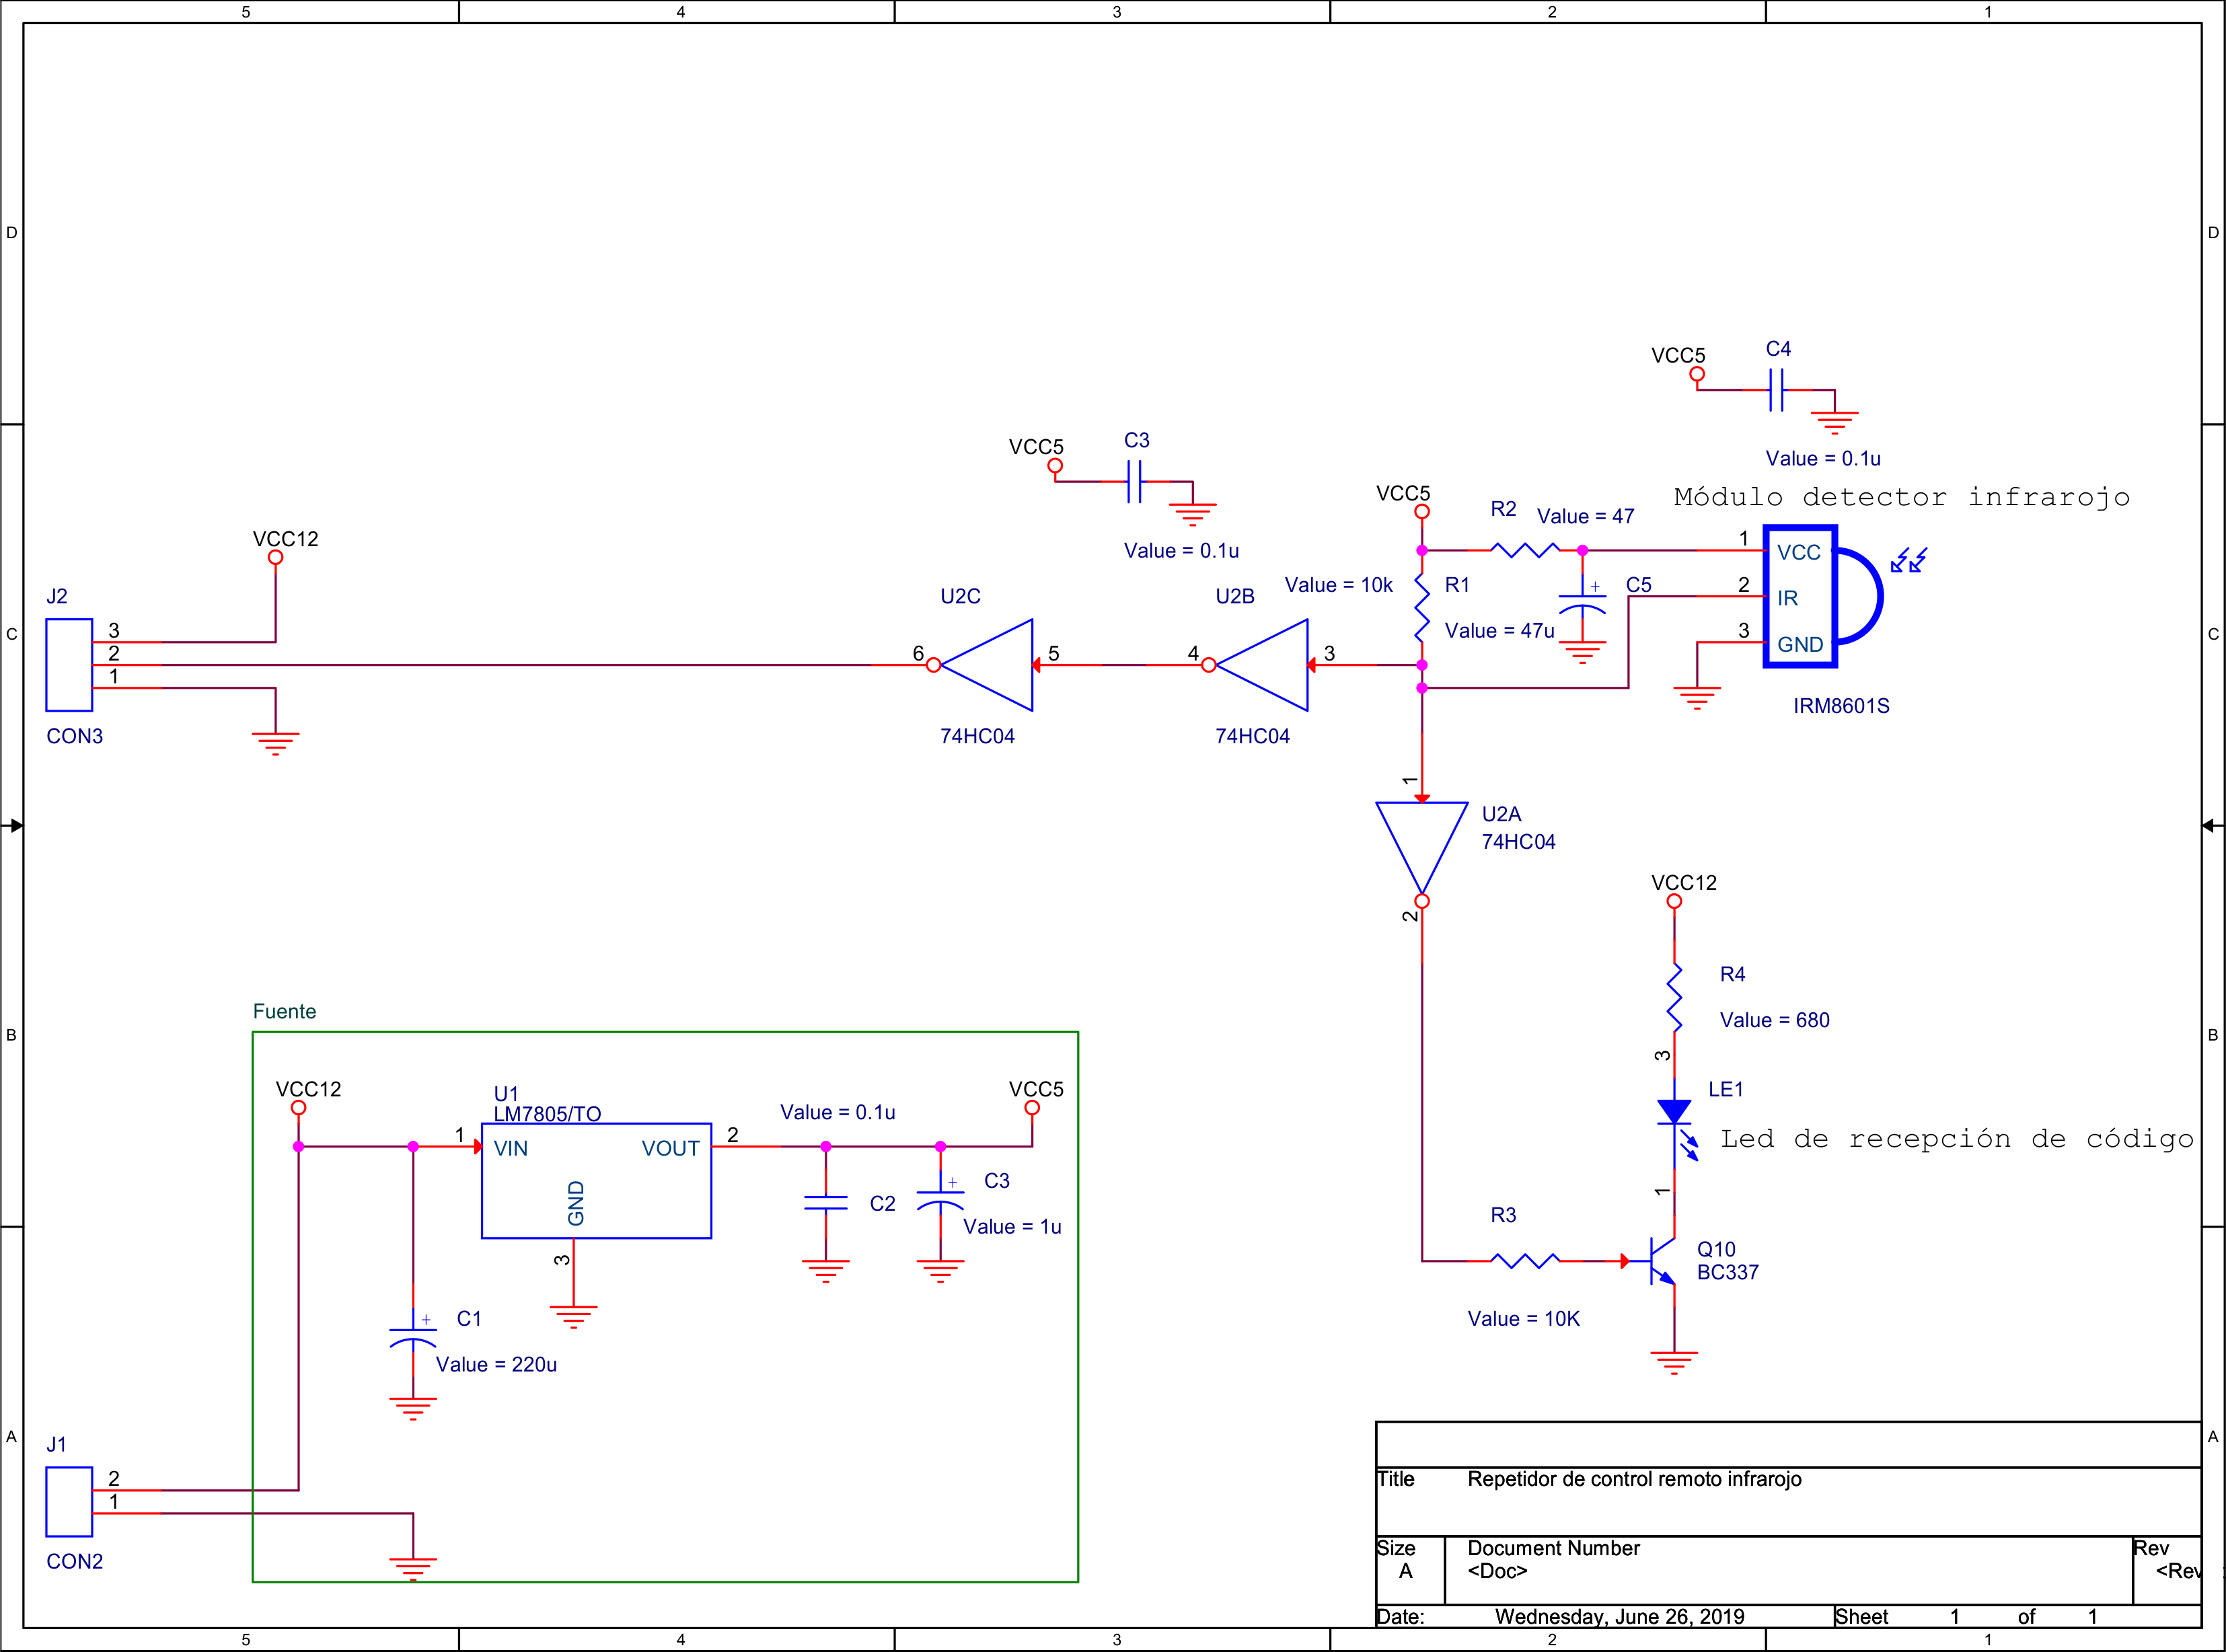
\includegraphics[width=0.9\paperwidth, angle=90]{img/SCH/receiver.png}
	\caption{\footnotesize{Circuito receptor.}}
	\label{fig:IR_receiver_sch}
\end{figure}



\clearpage

\begin{figure}[H]
	\centering
	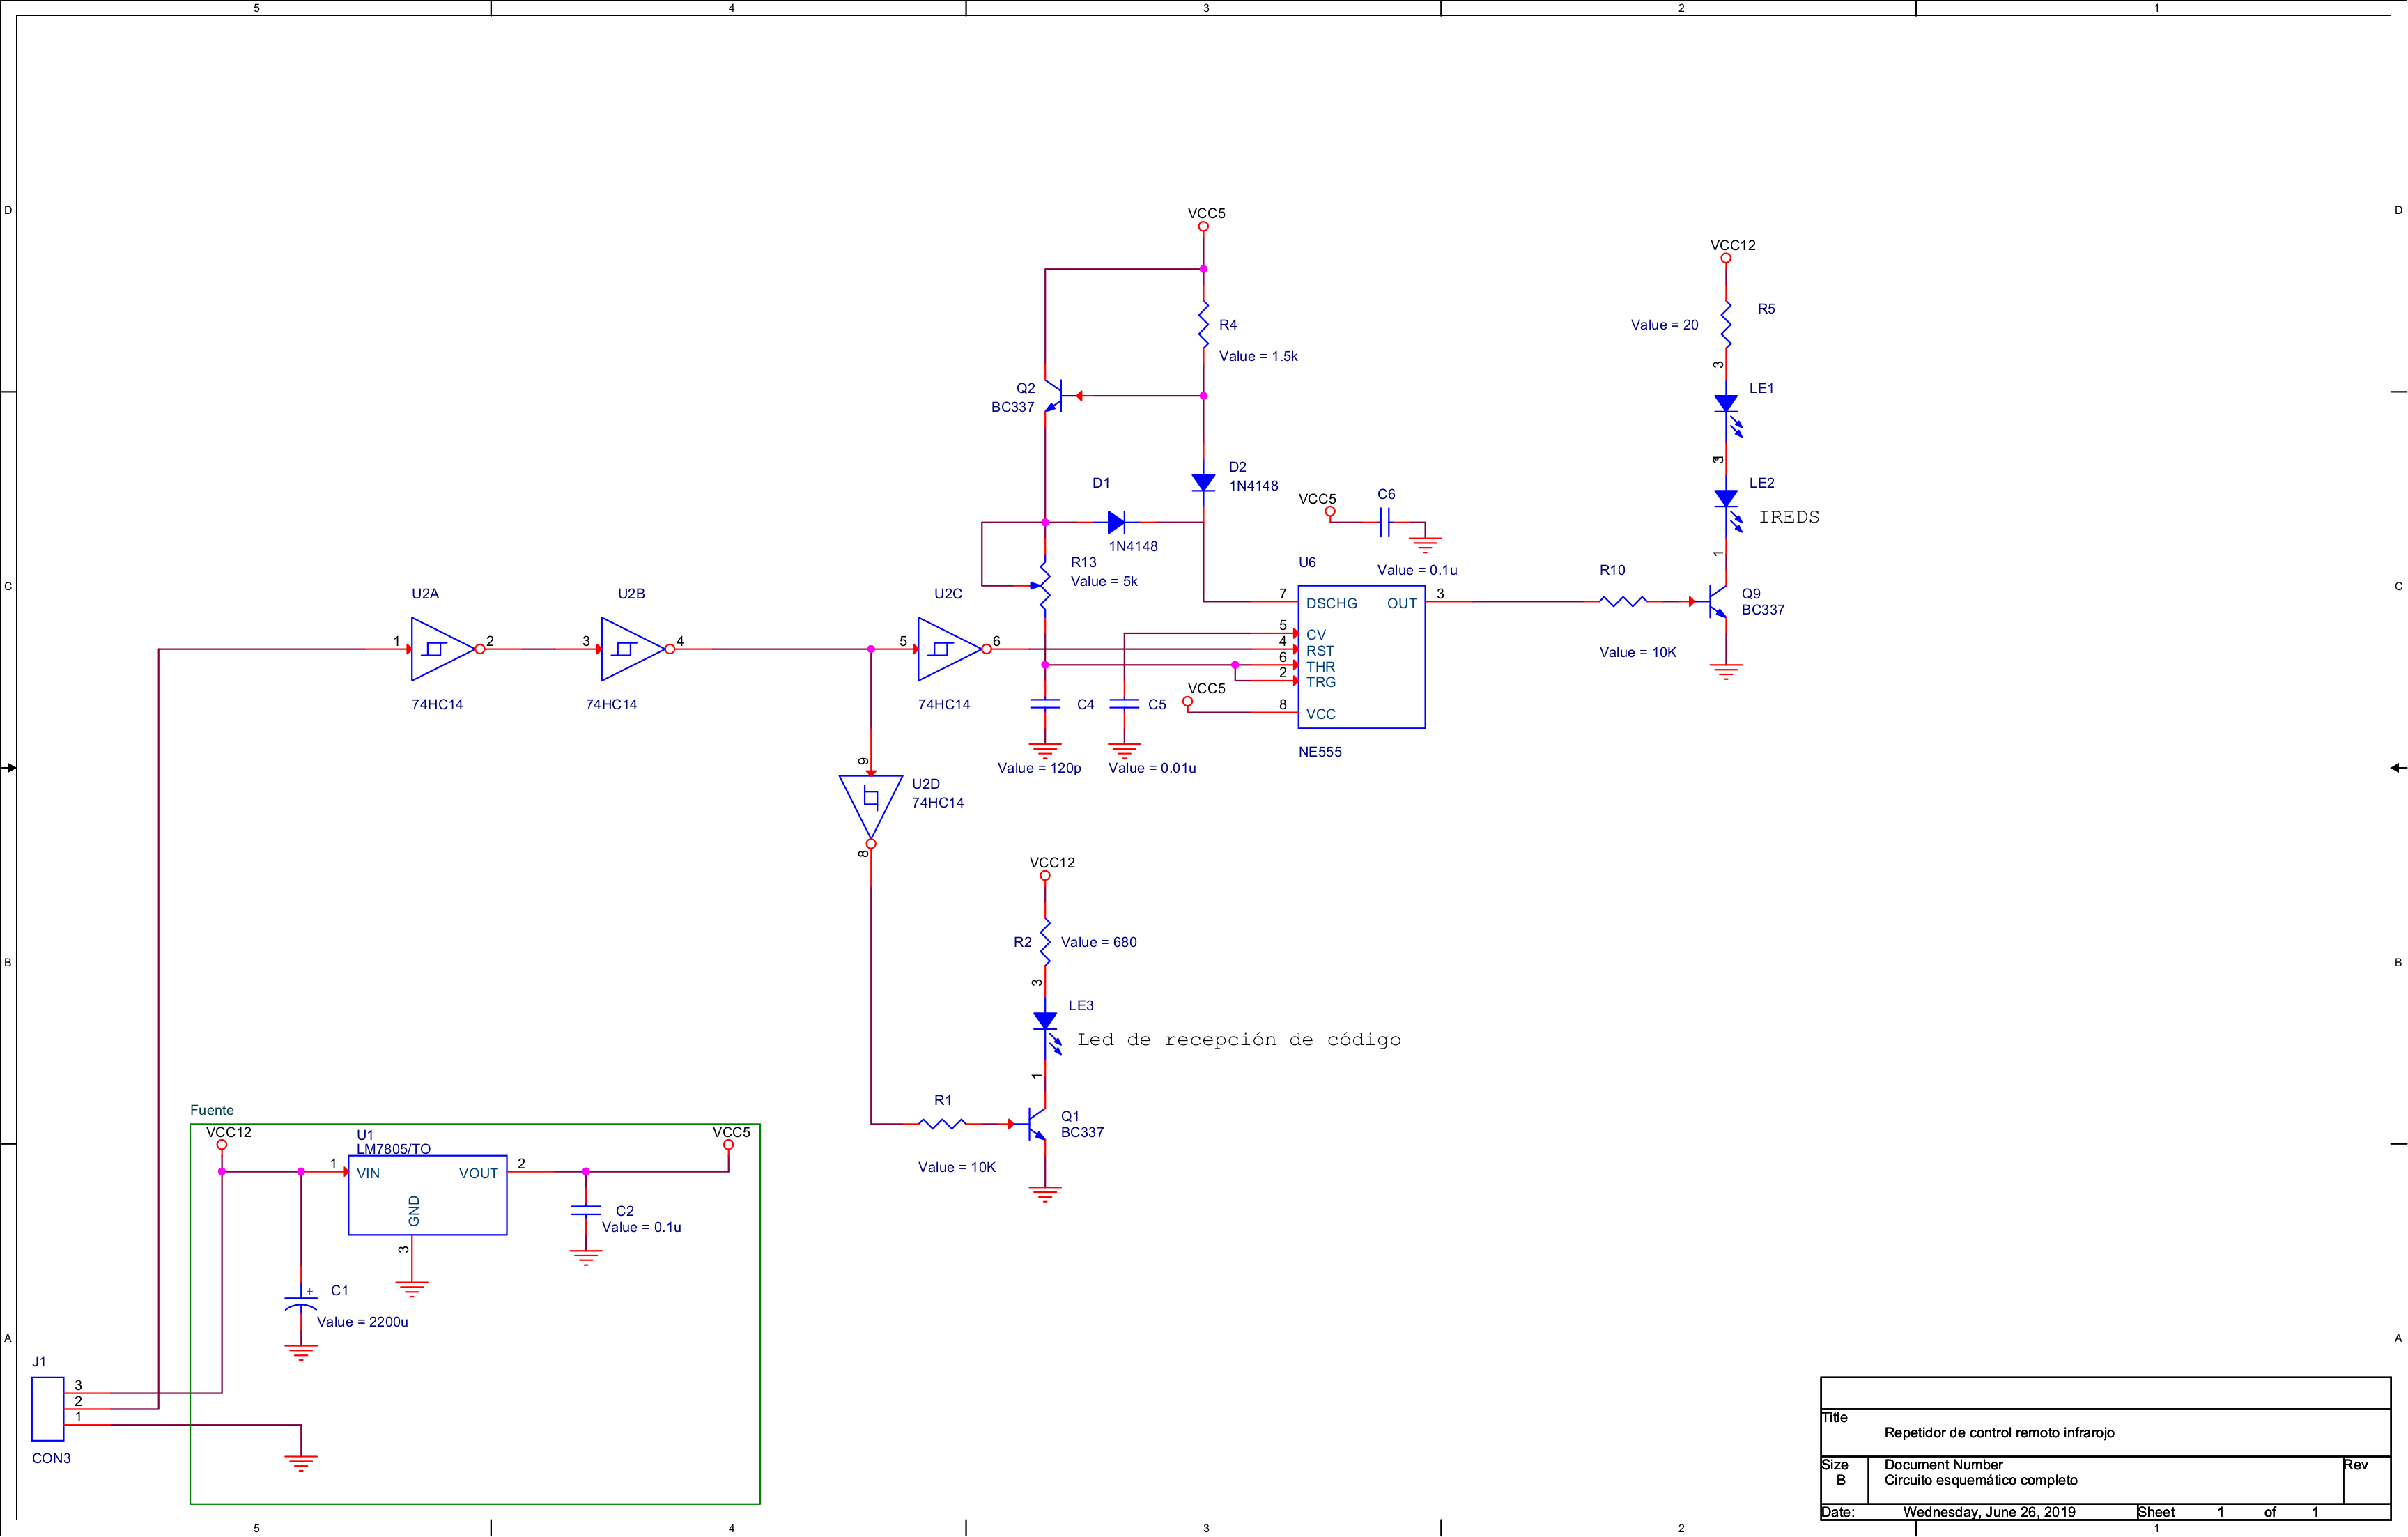
\includegraphics[width=0.9\paperwidth, angle=90]{img/SCH/transmitter.png}
	\caption{\footnotesize{Circuito transmisor.}}
	\label{fig:IR_transmitter_sch}
\end{figure}


\clearpage